\themaG
\graphicspath{{../Ch7_Position_relative_de_deux_droites/Images/}}

\chapter{Position relative\\de deux droites}
\label{C04}

%%%%%%%%%%%%%%%%%%%%%%%%%%%%%%%%%%%%%%%%%%
\begin{prerequis}[Connaissances et compétences abordées]
   \begin{itemize}
      \item Perpendicularité, parallélisme.
   \end{itemize}
\end{prerequis}

\vfill

\begin{debat}[Débat : un peu de vocabulaire] 
   {\bf Perpendiculaire} : chez les Romains, {\it perpendiculum} désigne le fil à plomb ; en ancien français, un {\it perpendicle} est aussi un fil à plomb mais signifie également verticale et ce n'est  que dans la deuxième moitié du {\small XVI}\up{e} siècle que le mot {\it perpendiculaire} prend le sens que nous connaissons actuellement. \\
   {\bf Parallèle} : chez les Grecs, {\it parallelos} signifie \og placé en regard \fg{} et désigne aussi des cercles concentriques. Le mot est formé à partir de {\it para}, \og à côté \fg{} et de {\it allelon}, \og les uns et les autres \fg{}. Le mot parallèle est introduit au {\small XVI}\up{e} siècle dans le vocabulaire mathématique.
   {\centerline{\footnotesize\it Source : Les mots et les maths, Bertrand Hauchecorne, ellipses poche 2014.}}
   \begin{center}
      \begin{pspicture}(0,-0.5)(5,2.5)
         \psset{linecolor=B1,linewidth=1mm}
         \psline(0,0)(2,0)
         \psline(1,0)(1,2)
         \psline(3.5,0)(4.5,2)
         \psline(4,0)(5,2)
      \end{pspicture}
   \end{center}
   \begin{cadre}[B2][F4]
      \begin{center}
         Vidéo : \href{https://lesfondamentaux.reseau-canope.fr/video/reconnaitre-des-droites-perpendiculaires.html}{\bf Reconnaître des droites perpendiculaires}, et \href{https://lesfondamentaux.reseau-canope.fr/video/reconnaitre-des-droites-paralleles.html}{\bf Reconnaître des droites parallèles} du site {\it Canopé}, épisode de la série {\it Les fondamentaux}.
      \end{center}
   \end{cadre}
\end{debat}

\vfill

\textcolor{PartieGeometrie}{\large\sffamily\bfseries Cahier de compétences} : chapitre 7, exercices 1. 

%%%%%%%%%%%%%%%%%%%%%%%%%%%%%%%%%%%%
%%%%%%%%%%%%%%%%%%%%%%%%%%%%%%%%%%%%%
\activites

\begin{activite}[D'équerre ou pas d'équerre ?]
   {\bf Objectifs :} repérer des angles droits ; utiliser des instruments pour vérifier qu'un angle est droit ; coder une figure.
   \begin{QCM}
      \partie[construction d'un gabarit d'angle droit en papier]
         Pour vérifier qu'un angle est droit, on peut utiliser une équerre, mais il est facile de construire un gabarit d'angle droit avec un simple morceau de papier :
         \begin{center}
            \begin{pspicture}(0,0)(4,4.5)
               \psline(0,4)(0,1.5)(4,1.5)(4,3.5)
               \pslineByHand(0,4)(4,3.5)
               \rput(2,1){prendre un morceau}
               \rput(2,0.6){de papier}
            \end{pspicture}
            \begin{pspicture}(0,0)(3.5,4.5)
               \psline(1,4)(1,2.85)
               \psline(1,2.4)(1,1.5)(2.5,1.5)(3,3.5)
               \psline(2.5,1.5)(0.8,2.5)(1.8,4.2)
               \pslineByHand(1,4)(1.65,3.9)
               \pslineByHand(3,3.5)(1.75,4.25)
               \rput(2,1){le plier en deux}
               \rput(2,0.6){n'importe comment}
            \end{pspicture}
            \begin{pspicture}(0.5,0)(3.5,4.5)
               \pspolygon(3,3.5)(2.75,2.5)(1,3)(2,4.3)
               \psline(1,4)(1,3)(1.1,3.5)(1.35,3.46)
               \pslineByHand(1.65,3.9)(0.95,4)
               \rput(2,1.4){le replier en}
               \rput(2,1){suivant la}
              \rput(2,0.6){première pliure}
            \end{pspicture}
            \begin{pspicture}(0.5,0)(3.5,4.5)
               \pspolygon(3,3.5)(2.75,2.5)(1,3)(2,4.3)
               \psline(1,4)(1,3)(1.1,3.5)(1.35,3.46)
               \pspolygon[fillstyle=solid,fillcolor=black](2.75,2.5)(2.8,2.7)(2.6,2.755)(2.55,2.56)
               \pslineByHand(1.65,3.9)(0.95,4)
               \rput(2,1){marquer}
               \rput(2,0.6){l'angle droit}
            \end{pspicture}
         \end{center}
         
      \partie[angle droit ou pas ?]    
         Marquer les angles droits de cette figure : combien y en a-t-il ? \pf
         \begin{center}
            \begin{pspicture}(0,-0.5)(14,10.5)
               \pstGeonode[PointSymbol=none,PointName=none](4,0.5){Q}(6.5,0.4375){R}(10,1){C}(0.66,3.5){D}(6.5,3.5){E}(10,3.5){F}(13,3.5){G}(0.5,7.5){H}(5,7.5){I}(10,8){J}(13,8){K}(14,8.5){L}(6.5,8.5){M}(4.25,10.5){N}(7,9.5){O}
               \pstLineAB{Q}{R}
               \pstLineAB{R}{E}
               \pstLineAB{D}{G}
               \pstLineAB{C}{G}
               \pstLineAB{C}{J}
               \pstLineAB{J}{O}
               \pstLineAB{D}{H}
               \pstLineAB[nodesepB=2.36]{Q}{N}
               \pstLineAB[nodesepB=-0.87]{O}{M}
               \pstLineAB[nodesepB=0.62]{F}{L}
               \pstLineAB[nodesepB=-1.04]{F}{I}
               \pstLineAB[nodesepB=-0.62]{H}{K}
            \end{pspicture}
         \end{center}
      \end{QCM}
\end{activite}


%%%%%%%%%%%%%%%%%%%%%%%%%%%%%%%%%%%%%%%%%%
\cours 

%%%%%%%%%%%%%%%%%%%%%%%%%%%%%%%%%%%%%%%
%%%%%%%%%%%%%%%%% I %%%%%%%%%%%%%%%
\section{Droites perpendiculaires}

\begin{definition}
   Lorsque deux droites forment un angle droit, on dit qu'elles sont \textbf{perpendiculaires}.
\end{definition}

\begin{exemple}
   \begin{pspicture}(-1.5,-0.5)(4,3)
      \psline(0,0)(4,2)
      \psline(2.5,0)(1,3)
      \pspolygon[linecolor=A1](2,1)(2.25,1.125)(2.125,1.375)(1.875,1.25)
      \equerre{2}{1}{116.5}{1}
      \rput(3.8,1.6){$(d)$}
      \rput(1.5,2.9){$(\Delta)$}
   \end{pspicture}
   \correction
      Les deux droites $(d)$ et $(\Delta)$ sont perpendiculaires. \\
      On peut le constater par exemple à l'aide d'une équerre. \\
      On code grâce à un petit carré au niveau de l'angle droit. \\ [5mm]
      On note \fbox{$(d)\perp(\Delta)$}
\end{exemple}

   
%%%%%%%%%%%%%%%%% 2 %%%%%%%%%%%%%%%
\section{Droites parallèles}

\begin{definition}
   Lorsque deux droites ne se coupent pas, on dit qu'elles sont \textbf{parallèles}.
\end{definition}

\begin{exemple}
   \begin{pspicture}(-1.5,-0.5)(4,3)
      \psline(0,0)(4,2)
      \psline(-0.5,0.7)(3.5,2.7)
      \rput(3.8,1.4){$(d)$}
      \rput(3.4,2.3){$(d')$}
   \end{pspicture}
   \correction
      Les deux droites $(d)$ et $(d')$ sont parallèles. \\ [5mm]
      On note \fbox{$(d)\sslash(d')$}      
\end{exemple}

   
%%%%%%%%%%%%%%%%% I %%%%%%%%%%%%%%%
\section{Position relative de deux droites}

On peut résumer la position relative de deux droites selon l'organigramme suivant :

\begin{center}
   \pstree[levelsep=20mm,labelsep=1mm,treesep=15mm]{
   \TR{\fbox{Position relative de deux droites}}}
      {\pstree{\TR{\fbox{Sécantes}}}
	  {\TR{\fbox{Perpendiculaires}}\taput{$\perp$}	
           \TR{\fbox{Non perpendiculaires}}\taput{$\not\perp$}	   
	  }
      \pstree{\TR{\fbox{Parallèles}}}
	  {\TR{\fbox{Confondues}}\taput{$\infty$}
	   \TR{\fbox{Distinctes}}\taput{$0$}
	  }	
      }
   \end{center} 


%%%%%%%%%%%%%%%%%%%%%%%%%%%%%%%%%%%%%%%%%%
\exercicesbase

\begin{colonne*exercice}

\serie{Droites perpendiculaires et parallèles}

\begin{exercice}
   Pour chaque paire de droites suivantes, dire si elles semblent sécantes ou parallèles puis préciser si elles semblent perpendiculaires ou non, confondues ou distinctes. Vérifier avec les instruments.
   \begin{center}
   \psset{unit=0.9}
   \small
      \begin{pspicture}(0,0.5)(8,5.3)
         \small
         \psline(1,1)(7.5,1)
         \psline(1,1)(5,5)
         \psline(3,1)(6,4)
         \psline(4,4)(7.5,0.5)
         \psline(0,3)(8,3)
         \rput(0.7,0.7){A}
         \rput(3,0.7){B}
         \rput(7,0.7){C}
         \rput(0,2.7){D}
         \rput(3,2.7){E}
         \rput(5,2.7){F}
         \rput(8,2.7){G}
         \rput(4,3.7){H}
         \rput(6.3,4.3){I}
         \rput(5,4.7){J}        
      \end{pspicture}
   \end{center}
   \begin{colenumerate}{3}
      \item (AJ) et (FC)
      \item (EH) et (BF)
      \item (DE) et (FG)
      \item (AB) et (BF)
      \item (IF) et (HC)
      \item (DG) et (AJ)
   \end{colenumerate}
\end{exercice}

\medskip

\begin{exercice}
   En utilisant le quadrillage, nommer les droites parallèles et les droites perpendiculaires.
   \begin{center}
   \psset{unit=0.45}
   \small
      \begin{pspicture}(0,0)(18,13)
         \psgrid[gridlabels=0,subgriddiv=0,gridcolor=lightgray](18,13)
         \psline(5,0)(18,13)
         \psline(15,0)(2,13)
         \psline(16,0)(0,5.33)
         \psline(0,4)(9,13)
         \psline(18,4)(0,10)
         \pstGeonode[PosAngle=-90](8,12){A}(3,9){B}(12,6){C}(10,5){D}(1,5){E}(6,1){F}(10,2){G}(7.5,7.5){H}
      \end{pspicture}
   \end{center}
\end{exercice}

\smallskip

\begin{exercice}
   Complète avec les signes $\perp$ ou $\sslash$.
   \begin{colenumerate}{2}
      \item (AB) \dots{} \dots (BC)
      \item (AB) \dots{} \dots (DE)
      \item (BC) \dots{} \dots (DE)
      \item (BD) \dots{} \dots (DF)
      \item (EF) \dots{} \dots (CD)
      \item (DF) \dots{} \dots (CE)
   \end{colenumerate}
   \begin{center}
   \psset{unit=0.8}
   \small
      \begin{pspicture}(0,0)(8,4)
      \psgrid[gridlabels=0,subgriddiv=0,gridcolor=lightgray](8,4)
         \psline(1,1)(3,1)(3,3)(5,3)(5,1)(7,1)
         \pstGeonode[PosAngle={-90,-90,90,90,-90,-90},PointSymbol=none](1,1){A}(3,1){B}(3,3){C}(5,3){D}(5,1){E}(7,1){F}
         \end{pspicture}
   \end{center}
\end{exercice}

\begin{exercice}
   Vrai ou faux ?
   \begin{enumerate}
      \item Trois droites deux à deux  sécantes sont concourantes.
      \item Deux droites non parallèles sont sécantes.
      \item Deux droites peuvent avoir exactement trois points communs.
      \item Deux droites non perpendiculaires sont sécantes.
   \end{enumerate}
\end{exercice}

\smallskip

\begin{exercice}
   Dans cette figure, les droites qui semblent perpendiculaires ou parallèles le sont réellement. Déterminer :
   \begin{enumerate}
      \item La droite perpendiculaire à (HK) passant par H.
      \item La droite perpendiculaire à (CE) passant par N.
      \item La droite parallèle à (HP) passant par N.
      \item La droite parallèle à (CF) passant par S.
      \item Le droite parallèle à (PN) passant par R.
   \end{enumerate}
   \begin{center}
   \psset{unit=0.8}
      \begin{pspicture}(-0.5,0)(8.5,4)
         \small
         \psframe(0,0)(8,4)
         \psframe(2,1)(6,3)
         \pspolygon(4,0)(8,2)(4,4)(0,2)
         \psline(0,4)(8,0)
         \psline(0,0)(8,4)
         \pstGeonode[PosAngle={-135,-90,-45,-90,-90,180,90,0,90,90,135,90,45},PointSymbol=none](0,0){E}(4,0){C}(8,0){F}(2,1){Y}(6,1){P}(0,2){R}(4,2){L}(8,2){N}(2,3){H}(6,3){K}(0,4){D}(4,4){S}(8,4){G}
         \end{pspicture}
   \end{center}
\end{exercice}

\begin{exercice}
   À l'aide de la figure, répondre aux questions.
   \begin{center}
      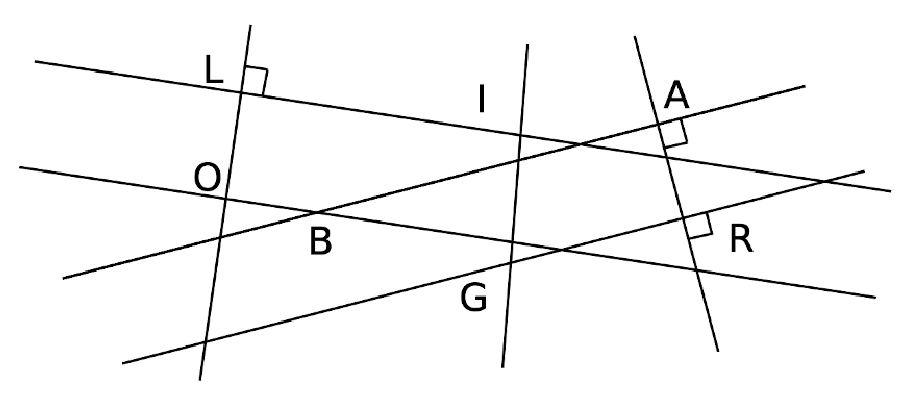
\includegraphics[width=8cm]{exercice}
   \end{center}
   \begin{enumerate}
      \item Quelles sont les droites qui sont perpendiculaires ?
      \item Quelle semble être la position relative des droites (BA) et (GR) ?
      \item Quelle est la droite perpendiculaire à la droite (GR) passant par le point A ?
      \item Quelle est la droite perpendiculaire à la droite (AR) passant par le point B ?
      \item Quelle est la droite perpendiculaire à la droite (LO) passant par le point I ?
   \end{enumerate}
\end{exercice}
\flushright{\it\footnotesize Source : Sesamath, le manuel 6\up{e}. Génération 5 - 2013}
\end{colonne*exercice}


%%%%%%%%%%%%%%%%%%%%%%%%%%%%%%%%%%%%%%%
%%%%%%%%%%%%%%%%%%%%%%%%%%%%%%%%%%%%%%%
\Recreation

\enigme[La grenouille qui saute]
   Prendre une feuille dont la longueur est deux fois plus longue que la largeur. \\
   Les plis en courts pointillés sont des plis \og vallée \fg, les plis en longs pointillés sont des plis \og montagne \fg. \\
   {\small
   \psset{linecolor=PartieStatistique}
   \begin{tabular}{p{3.8cm}p{3.8cm}p{3.8cm}p{3.8cm}}
      \begin{pspicture}(0.1,-0.25)(3.9,4.5)
         \psframe(1,0)(3,4)
         \psline[linestyle=dotted](1,2)(3,2)
         \rput(0.7,2){\textcolor{PartieStatistique}{A}}
         \rput(3.3,2){\textcolor{PartieStatistique}{B}}
      \end{pspicture}
      &
      \begin{pspicture}(0.1,-0.25)(3.9,4.5)
         \psframe(1,0)(3,4)
         \psline[linestyle=dotted](1,2)(3,2)
         \psline[linestyle=dotted](1,2)(3,4)
         \rput(0.7,2){\textcolor{PartieStatistique}{A}}
         \rput(3.3,2){\textcolor{PartieStatistique}{B}}
      \end{pspicture}
      &
      \begin{pspicture}(0.1,-0.25)(3.9,4.5)
         \psframe(1,0)(3,4)
         \psline[linestyle=dotted](1,2)(3,2)
         \psline[linestyle=dotted](1,2)(3,4)
         \psline[linestyle=dotted](1,4)(3,2)
         \psline[linestyle=dotted](1,0)(3,2)
         \psline[linestyle=dotted](1,2)(3,0)
          \rput(0.7,2){\textcolor{PartieStatistique}{A}}
         \rput(3.3,2){\textcolor{PartieStatistique}{B}}
      \end{pspicture}
      &
      \begin{pspicture}(0.1,-0.25)(3.9,4.5)
         \psframe(1,0)(3,4)
         \psline[linestyle=dotted](1,2)(3,2)
         \psline[linestyle=dotted](1,2)(3,4)
         \psline[linestyle=dotted](1,4)(3,2)
         \psline[linestyle=dotted](1,0)(3,2)
         \psline[linestyle=dotted](1,2)(3,0)
         \psline[linestyle=dashed](1,3)(3,3)
         \psline[linestyle=dashed](1,1)(3,1)
         \rput(0.7,3){\textcolor{PartieStatistique}{C}}
         \rput(3.3,3){\textcolor{PartieStatistique}{D}}
         \rput(0.7,2){\textcolor{PartieStatistique}{A}}
         \rput(3.3,2){\textcolor{PartieStatistique}{B}}
         \rput(0.7,1){\textcolor{PartieStatistique}{E}}
         \rput(3.3,1){\textcolor{PartieStatistique}{F}}
      \end{pspicture} \\
      1) Plier la feuille en deux selon la médiane la plus courte du rectangle : (AB)
      &
      2) Dans le carré du haut, plier suivant la diagonale passant par A puis déplier
      &
      3) Plier puis déplier de la même manière les trois autres diagonales
      &
      4) Plier suivant les médianes (CD) et (EF) des deux carrés \\
      \begin{pspicture}(0.1,-0.25)(3.9,3.5)
         \psframe(1,0)(3,2)
         \psline[linestyle=dotted](1,0)(3,2)
         \psline[linestyle=dotted](1,2)(3,0)
         \psline[linestyle=dashed](1,1)(3,1)
         \rput(0.7,2){\textcolor{PartieStatistique}{\footnotesize A}}
         \rput(3.3,2){\textcolor{PartieStatistique}{\footnotesize B}}
         \rput(0.7,1){\textcolor{PartieStatistique}{\footnotesize E}}
         \rput(3.3,1){\textcolor{PartieStatistique}{\footnotesize F}}      
         \psline(3,2)(2,3)(1,2)
         \psdot(2,2)
         \rput(2,1.7){\textcolor{PartieStatistique}{\footnotesize C}}
         \rput(2,2.3){\textcolor{PartieStatistique}{\footnotesize D}}    
      \end{pspicture}
      &
      \begin{pspicture}(0.1,-0.25)(3.9,3.5)
         \pspolygon(2,1)(3,2)(2,3)(1,2)
         \psline(1,2)(3,2)
         \psdot(2,2)
         \rput(1.85,1.8){\textcolor{PartieStatistique}{\footnotesize C}}
         \rput(1.85,2.2){\textcolor{PartieStatistique}{\footnotesize D}}
         \rput(2.15,1.8){\textcolor{PartieStatistique}{\footnotesize E}}
         \rput(2.15,2.2){\textcolor{PartieStatistique}{\footnotesize F}}
         \rput(0.8,2){\textcolor{PartieStatistique}{\footnotesize A}}
         \rput(3.2,2){\textcolor{PartieStatistique}{\footnotesize B}}    
      \end{pspicture}
      &
      \begin{pspicture}(0.1,-0.25)(3.9,3.5)
         \pspolygon(2,1)(3,2)(2,3)(1,2)
         \psline(1,2)(3,2)
         \psline[linestyle=dotted](2,2)(2.5,2.5)
         \rput(0.8,2){\textcolor{PartieStatistique}{\footnotesize A}}
         \rput(3.2,2){\textcolor{PartieStatistique}{\footnotesize B}}
         \rput(2,3.2){\textcolor{PartieStatistique}{\footnotesize G}}
         \psarc[linecolor=cyan]{->}(2.6,2.6){0.35}{-45}{135}
     \end{pspicture}
      &
      \begin{pspicture}(0.1,-0.25)(3.9,3.5)
         \pspolygon(2,1)(3,2)(2,3)(1,2)
         \psline(1,2)(3,2)
         \psline(2.5,1.5)(1.5,2.5)
         \psline(1.5,1.5)(2.5,2.5)
         \psline(2,1)(2,3)
      \end{pspicture} \\
      5) Joindre les points C et D l'un contre l'autre et les rabattre sur la droite (AB)
      &
      6) Faire la même chose avec les points E et F
      &
      7) Rabattre le coin B supérieur droit sur le sommet G
      &
      8) Faire de même avec les trois autres coins en A et B \\
      \begin{pspicture}(0.1,0.75)(3.9,3.5)
         \pspolygon(2,1)(3,2)(2,3)(1,2)
         \psline(1,2)(3,2)
         \psline(2.5,1.5)(1.5,2.5)
         \psline(1.5,1.5)(2.5,2.5)
         \psline(2,1)(2,3)
         \psline[linestyle=dotted](2,2)(2.29,2.71)
         \psarc[linecolor=cyan]{<-}(2.35,2.75){0.2}{-40}{130}
      \end{pspicture}
      &
      \begin{pspicture}(0.1,0.75)(3.9,3.5)
         \pspolygon(2,1)(3,2)(2,3)(1,2)
         \psline(1,2)(3,2)
         \pspolygon[fillstyle=solid,fillcolor=white](1.29,1.29)(1.71,1.29)(2.29,2.71)(2.71,2.71)
         \pspolygon[fillstyle=solid,fillcolor=white](1.29,2.71)(1.7,2.71)(2.29,1.29)(2.71,1.29)
     \end{pspicture}
      &
     \begin{pspicture}(0.1,0.75)(3.9,3.5)
         \pspolygon(1.29,1.29)(1.71,1.29)(2.29,2.71)(2.71,2.71)
         \pspolygon(1.29,2.71)(1.7,2.71)(2.29,1.29)(2.71,1.29)
         \pspolygon[fillstyle=solid,fillcolor=white](2,1)(3,2)(2,3)(1,2)
         \psline[linestyle=dotted](2,1)(2,3)
         \psline[linestyle=dashed](1,2)(3,2)
         \rput(2,3.2){\textcolor{PartieStatistique}{\footnotesize G}}
         \rput(2,0.8){\textcolor{PartieStatistique}{\footnotesize H}}
      \end{pspicture}
      &
      \begin{pspicture}(0.1,0.75)(3.9,3.5)
         \pspolygon(1.29,1.29)(1.71,1.29)(2.29,2.71)(2.71,2.71)
         \pspolygon(1.29,2.71)(1.7,2.71)(2.29,1.29)(2.71,1.29)
         \pspolygon[fillstyle=solid,fillcolor=white](2,1)(3,2)(2,3)(1,2)
         \psline[linestyle=dotted](2,1)(2,3)
         \psline[linestyle=dotted](1.42,1.58)(2,3)
         \psline[linestyle=dotted](2.58,1.58)(2,3)
         \rput(2,3.2){\textcolor{PartieStatistique}{\footnotesize G}}
         \rput(2,0.8){\textcolor{PartieStatistique}{\footnotesize H}}
         \rput(0.8,2){\textcolor{PartieStatistique}{\footnotesize B}}
         \rput(3.2,2){\textcolor{PartieStatistique}{\footnotesize A}}
         \psarc[linecolor=cyan]{<-}(2.5,2.1){0.35}{200}{-20}
         \psarc[linecolor=cyan]{->}(1.5,2.1){0.35}{200}{-20}
      \end{pspicture} \\
      9) Replier le triangle supérieur droit de manière à superposer son hypoténuse à son côté inférieur
      &
      10) Faire la même chose avec les trois autres triangles
      &
      11) Retourner la feuille, plier puis déplier suivant la diagonale (GH)
      &
      12) Amener les points A et B sur la diagonale (GH) \\ 
       \begin{pspicture}(0.1,0.75)(3.9,3.5)
         \pspolygon(1.29,1.29)(1.71,1.29)(2.29,2.71)(2.71,2.71)
         \pspolygon(1.29,2.71)(1.7,2.71)(2.29,1.29)(2.71,1.29)
         \pspolygon[fillstyle=solid,fillcolor=white](2,2)(2.5,2.5)(2,3)(1.5,2.5)
         \pspolygon[fillstyle=solid,fillcolor=white](2,1)(2.58,1.58)(2,3)(1.42,1.58)
         \psline[linestyle=dotted](2,1)(2,1.58)
         \psline(2,1.58)(2,3)
         \psline(1.42,1.58)(2.58,1.58)
         \psline(1.58,2)(2,1.58)(2.42,2)
         \psline[linestyle=dotted](1.5,1.48)(2.5,1.48)
         \psarc[linecolor=cyan]{<-}(1.9,1.58){0.5}{80}{-80}
      \end{pspicture}
      &
      \begin{pspicture}(0.1,0.75)(3.9,3.5)
         \pspolygon(1.29,1.29)(1.71,1.29)(2.29,2.71)(2.71,2.71)
         \pspolygon(1.29,2.71)(1.7,2.71)(2.29,1.29)(2.71,1.29)
         \pspolygon[fillstyle=solid,fillcolor=white](2,2)(2.5,2.5)(2,3)(1.5,2.5)
         \pspolygon[fillstyle=solid,fillcolor=white](1.5,1.5)(2.5,1.5)(2.58,1.58)(2,3)(1.42,1.58)
         \psline(2,1.58)(2,3)
         \psline(1.42,1.58)(2.58,1.58)
         \psline(1.58,2)(2,1.58)(2.42,2)
         \pspolygon[fillstyle=solid,fillcolor=white](1.5,1.5)(2.5,1.5)(2,2)
         \psline(1.71,1.29)(1.5,1.5)
         \psline(2.29,1.29)(2.5,1.5)
         \psline[linecolor=cyan]{->}(1.7,2.1)(1.95,1.7)
         \psline[linecolor=cyan]{->}(2.3,2.1)(2.05,1.7)
      \end{pspicture}
      &
      \begin{pspicture}(0.1,0.75)(3.9,3.5)
         \pspolygon(1.29,1.29)(1.71,1.29)(2.29,2.71)(2.71,2.71)
         \pspolygon(1.29,2.71)(1.7,2.71)(2.29,1.29)(2.71,1.29)
         \pspolygon[fillstyle=solid,fillcolor=white](2,2)(2.5,2.5)(2,3)(1.5,2.5)
         \pspolygon[fillstyle=solid,fillcolor=white](1.5,1.5)(2.5,1.5)(2.58,1.58)(2,3)(1.42,1.58)
         \psline(2,1.58)(2,3)
         \psline(1.42,1.58)(2.58,1.58)
         \psline(1.58,2)(2,1.58)(2.42,2)
         \pspolygon[fillstyle=solid,fillcolor=white](1.5,1.5)(2.5,1.5)(2,2)
         \psline(1.71,1.29)(1.5,1.5)
         \psline(2.29,1.29)(2.5,1.5)
        \psline[linestyle=dashed](1.58,2)(2.42,2)
         \psline[linestyle=dotted](1.48,1.75)(2.52,1.75)
         \psarc[linecolor=cyan]{<-}(2.9,1.7){0.15}{80}{-80}
         \psarc[linecolor=cyan]{->}(2.7,2.1){0.15}{-100}{100}
      \end{pspicture}
      &
      \begin{pspicture}(0.1,0.75)(3.9,3.5)
         \pspolygon(2,2.05)(2.29,2.71)(2.71,2.71)
         \pspolygon(1.29,2.71)(1.7,2.71)(2,2.05)
         \pspolygon(1.48,2.24)(2.52,2.24)(2.42,2)(1.58,2)
        \pspolygon(1.48,2.24)(1.41,2.08)(1.5,2)(2.5,2)(2.59,2.08)(2.52,2.24)
         \psline(1.41,2.08)(1.54,2.08)
         \psline(2.59,2.08)(2.46,2.08)
         \psline(1.5,2)(1.55,2.06)
         \psline(2.5,2)(2.45,2.06)      
         \pspolygon[fillstyle=solid,fillcolor=white](2,2)(2.5,2.5)(2,3)(1.5,2.5)
         \pspolygon[fillstyle=solid,fillcolor=white](1.58,2)(2,3)(2.42,2)
         \psline(2,2)(2,3)
         \psline(1.79,2)(1.72,1.79)(1.5,2)(1.32,1.79)(1.72,1.79)
         \psline(2.21,2)(2.28,1.79)(2.5,2)(2.68,1.79)(2.28,1.79)  
      \end{pspicture}
       \\
      13) Plier le triangle inférieur au niveau des pattes de derrière
      &
      14) Rentrer les coins dans les encoches du triangle plié
      &
      15) Faire un pli montagne au niveau du sommet du triangle inférieur puis un pli vallée entre ce pli et la base &
      16) On obtient une jolie grenouille\dots{} ou pas ! \\
   \end{tabular}}

   Il ne reste plus qu'à décorer la grenouille ;-)

%\enigme[Pythagorea]
%   \partie[introduction]
%      {\bf Pythagorea} est un jeu géométrique qui propose de résoudre des problèmes à l’aide d’un quadrillage de manière graduée. Les notions abordées trouvent des applications dans toutes les classes de collège notamment : longueurs et distances, parallèles, triangles isocèles, médianes et milieux, symétrie axiale, perpendiculaires, parallélogrammes, trapèzes, carrés, cercles, symétrie centrale, théorème de Pythagore, longueurs et proportions, aire, triangles rectangles, hauteurs, losanges, rotation, angles\dots). \\
%      Il est possible de le télécharger gratuitement sur smartphones et tablettes sur l'\href{https://apps.apple.com/fr/app/pythagorea/id994864779}{App Store}{} ou sur \href{https://play.google.com/store/apps/details?id=com.hil_hk.pythagorea&hl=fr}{Google Play}.
%      
%   \partie[jouons !]
%      Deux \og thèmes \fg{} du jeu se rapportent à ce chapitre, il s'agit du thème 2 : Parallèles et du thème 6 : Perpendiculaires. \\
%      Voici résumé dans ce tableau les différentes \og missions \fg{} que l'on demande de résoudre :
%      \begin{center}
%         \begin{tabular}{|C{5}|C{5}|C{5}|}
%            \hline
%            \multicolumn{3}{|c|}{\bf Droites parallèles} \\
%            \hline
%            Construire une droite parallèle à une droite existante passant par un point donné. & Sélectionner deux droites parallèles parmi des droites données. & Construire deux droites parallèles passant par des paires de points donnés. \\
%            \includegraphics[width=4cm]{pythagorea_a1} & \includegraphics[width=4cm]{pythagorea_a2} & \includegraphics[width=4cm]{pythagorea_a3} \\
%            \hline
%            \hline
%            \multicolumn{3}{|c|}{\bf Droites perpendiculaires} \\
%            \hline
%            Construire une droite perpendiculaire à une droite existante passant par un point donné. & Sélectionner deux droites perpendiculaires parmi des droites données. & Construire deux droites perpendiculaires passant par des paires de points donnés. \\
%            \includegraphics[width=4cm]{pythagorea_e1} & \includegraphics[width=4cm]{pythagorea_e2} & \includegraphics[width=4cm]{pythagorea_e3} \\
%            \hline
%         \end{tabular}
%      \end{center}
 
